\section{Methodologies and Experiments}
\begin{figure}
    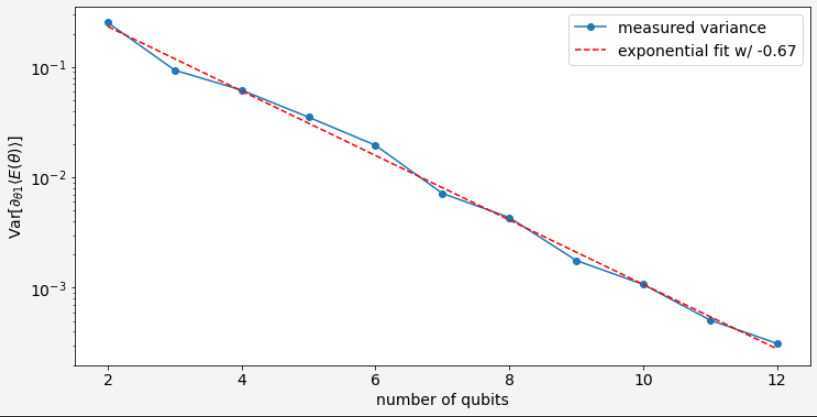
\includegraphics[width=\textwidth]{./ResearchDesign/Appendices/VarianceShrinking.png}
    \caption{
        An example of Barren Plateaus phenomenon occurs to a QNN model. 
        The variance of the gradient shrinking \textit{exponentially} with the number of qubits. 
        Barren Plateaus phenomenon prevents optimization algorithms to navigate the cost function landscape efficiently.
    }
    \label{Variance Shrinking demo}
\end{figure}

Cerezo et al. has pointed out that Barren Plateaus is cost function dependent \cite{cerezoCostFunctionDependent2021}, which implies that the only way to fully eliminate Barren Plateaus is to use a local cost function with a shallow circuit.
However, there are still other approaches to mitigate the phenomenon without using the local cost function.
Skolik et al. and Liu et al. \cite{skolikLayerwiseLearningQuantum2021, liuParameterInitializationMethod2021} suggest that we can initiate the starting parameters away from plateaus to guarantee the trainability from the first steps.
In this section, we design the methodologies to conduct the experiment to answer the research question.

\subsection{Research Type Overview}
In this experiment, we are use "top-down" approach, or "deductive research". 
We examine and implement the three theories \cite{cerezoCostFunctionDependent2021, liuParameterInitializationMethod2021, skolikLayerwiseLearningQuantum2021} as discussed in the literature review.
We then observe the data generated from the three approaches to compare them against the criteria as discussed.

\subsection{Research Strategy}
\textbf{In the first step, we create a QNN model to reproduce the Barren Plateaus.} 
We can use Qiskit to gain access to a wide range of ansatz, optimization algorithms, and most importantly the quantum emulator that capable of simulate up to 32 qubits.
The literature review had pointed out that the two factors causing Barren Plateaus are the \textit{ansatz depth, large number of qubits} and the \textit{randomised starting parameters}, so we configure the ansatz to have such characteristics.
Then we calculate the variance of the gradient, and notice if the variance is shrinking \textit{exponentially} with the number of qubits (see Figure \ref{Variance Shrinking demo}).
The result will be a QNN ansatz with the depth and number of qubit enough to produce the Barren Plateaus.

\textbf{In the second step, we implement the three approaches}.
The three methods as discussed in the literature review will be applied to the QNN model.
We will track the variances of the gradient for each method to identify if the model has mitigated the Barren Plateaus phenomenon.
The data of three models can be compared with criteria to identify their use cases:
\begin{itemize}
    \item How good the solution is;
    \item The size of the circuit;
    \item The size of the qubit registry;
    \item The time required to execute the circuit;
    \item The complexity of the algorithms.
\end{itemize}

\subsection{Sampling Strategy}
\begin{itemize}
    \item Probability Sampling: Random, representative sample of data
    \item Non-probability Sampling: non-random, non-representative
\end{itemize}

\subsection{Data Collecting Method}
Qualitative or Quantitative

\subsection{Resorces}
Most of our resources are open-sources
\begin{itemize}
    \item Python 3.6+: \url{https://www.python.org/downloads/}
    \item Anaconda: \url{https://www.anaconda.com/products/distribution}
    \item Jupyter Notebook: \url{https://jupyter.org/}
    \item Qiskit: \url{https://qiskit.org/}
    \item IBM Quantum: \url{https://quantum-computing.ibm.com/}
\end{itemize}